\section{CEGIS}
\label{sec:cegis}

Program se može sintetisati tako što se definišu njegove specifikacije i zapišu u vidu formule koja se prosledi SMT rešavaču (npr. Z3 [?]). SMT nađe valuaciju koja je zadovoljiva i to predstavlja rešenje. Problem nastaje u tome što formula koja se prosleđuje rešavaču sadrži univerzalne kvantifikatore koje usporavaju pretragu. Naime, rešavač bi u svakom slučaju pronašao rešenje za datu formulu, ali kako bi se to desilo u realnom vremenu, CEGIS (eng. \emph{Counterexample-Guided Inductive Synthesis}) u sebi sadrži posebne tehnike za optimizaciju.

Za većinu realnih problema nije neophodno da se razmatraju svi ulazi i izlazi kako bi se došlo do programa koji radi tačno za svaki od njih. Ovako razmišljajući, problem se menja i postaje: \emph{"koji je najmanji podskup ulaza koji je potrebno razmatrati da bi se sintetisao program koji zadovoljava date specifikacije?"}.

CEGIS upravo traga za tim minimalnim skupom. U petlji, korišćenjem SMT rešavača, on postepeno dolazi do svih mogućih implementacija že\-lje\-nog programa koristeći sve ulaze koji su razmatrani do tog trenutka (počinje sa 0 ulaza). U sledećoj iteraciji on razmatra dalje. Paralelno sa tim, drugim SMT rešavačem pronalazi kontra-primer koji pokazuje da poslednji sintetisani program nije rešenje. Ukoliko kontra-primer ne postoji, poslednji sintetisani program je rešenje. Ukoliko se prođe kroz sve iteracije i ne pronađe se rešenje, specifikacija programa nije smislena.

Jedna od mogućih implementacija se može naći na \cite{CEGISimpl}.


\subsection{Arhitektura}
\label{subsec:Arhitektura}

CEGIS se sastoji iz dve faze, induktivne sinteze i verifikacije. Na početku sintezeru dajemo specifikaciju željenog programa. U fazi sinteze pronalazi se program kandidat koji može da zadovolji specifikacije. Nakon toga se u fazi verifikacije proverava da li taj kandidat zaista zadovoljava specifikacije. Ako verifikator ne uspe da pronađe kontra primer znači da smo pronašli traženi program. U suprotnom, verifikator prosleđuje sintezeru informacije o kontra primeru, koje će mu pomoći prilikom daljeg traženja novog kandidata. Na slici \ref{fig:cegis} predstavljena je opšta arhitektura CEGIS-a.

Ovakav vid pretrage zove se pretraga vođena kontra primerima (eng. \emph{counterexample-guided}), zato što je povratna informacija sintezeru kontra primer koji se dodaje u specifikaciju programa \cite{PSE}. 

\begin{figure}[t]
    \begin{center}
        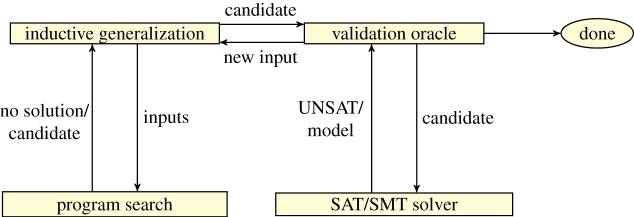
\includegraphics[scale=0.4]{resources/cegis.jpeg}
    \end{center}
    \caption{CEGIS petlja \cite{AboutPS}}
    \label{fig:cegis}
\end{figure}


Da bismo u potpunosti definisali CEGIS sintezu programa, potrebno je da odgovorimo na nekoliko važnih pitanja:

\begin{itemize}
    \item Kako treba da izgleda specifikacija traženog programa?
    \item Kako ćemo vršiti sintezu programa kandidata?
    \item Kako da proverimo da li program kandidat zadovoljava specifikacije?
    \item Kako da prosledimo povratne informacije za buduće kandidate?
\end{itemize}

\subsection{Primene CEGISa}
\label{subsec:PrimeneCEGISa}

U nastavku ćemo opisati kako se tri različite vrste sinteze programa koriste zajedno sa CEGIS idejom.


\subsubsection{Sinteza vođena oracle-om}
\label{subsec:OracleGuidedSynthesis}

Sinteza vođena oracle-om (eng. \emph{Oracle-guided synthesis}, u daljem tekstu \emph{OGS}) \cite{PSE} pretpostavlja da imamo implementaciju programa koji želimo da sintetišemo, koja se naziva oracle program. Mi ćemo oracle tretirati kao crnu kutiju, možemo da joj damo ulazne vrednosti i dobijemo odgovarajući izlaz, ali nećemo razmatrati njenu implementaciju. Počinjemo sa skupom test primera, koji su parovi ulaz-izlaz. Pošto imamo oracle, možemo da kreiramo novi test primer jednostavno generišući random ulaze i od oracla ćemo dobiti odgovarajući izlaz za svaki prosleđeni ulaz. Oracle program će predstavljati specifikaciju za OGS.


\subsubsection*{Faza sinteze}

OGS-u prosleđujemo biblioteku komponenti na osnovu koje sintezer kreira program koji je kandidat za rešenje. Faza sinteze će uzeti sve komponente i odlučiti kako da poveže njihove ulaze i izlaze tako da formiraju program. Ovako dobijem program će biti u SSA formi (eng. \emph{Static Single Assignment form} SSA) \cite{SSA}.

Na primer neka imamo biblioteku od tri komponente - dva sabiranja i jedno korenovanje. Njih je moguće povezati na sledeći način:

\begin{lstlisting}
program(x,y):
	o1 = add(x, y)
	o2 = add(o1, y)
	o3 = sqrt(o1)
	return o3
\end{lstlisting}

Primetimo da SSA forma jednostavno povezuje komponente me\-đu\-so\-bno, tako da ako želimo da imamo dva sabiranja moramo da obezbedimo dve komponente za sabiranje. Takođe primetimo da se vrednost $o2$ ne koristi, takozvani \emph{mrtvi kod}. U ovom slučaju to je poželjna karakteristika, jer ne moramo unapred tačno da odredimo koliko ćemo imati kojih operacija, već možemo samo da zadamo gornju granicu, a sintezer će generisati mrtvi kod za komponente koje se ne koriste.

Sintezer koristi test primere da ograniči broj načina na koje se komponente mogu povezati. On koristi SMT rešavač da odredi koje komponente da poveže kako bi program bio tačan za sve test primere. Ako SMT rešavač ne uspe da nađe rešenje, onda nijedan program koji koristi samo date komponente ne može da zadovolji sve test primere - komponente nisu dovoljne. U suprotnom vraća program u SSA formi koji zadovoljava sve test primere.


\subsubsection*{Faza verifikacije}

Ako postoji rešenje mi program koji je kandidat za rešenje prosleđujemo fazi verifikacije. Ovaj korak koristi SMT rešavač da odgovori na sledeće pitanje: Da li postoji program $P'$, različit od kandidata za rešenje $P$, koji takođe zadovoljava sve test primere, ali se na nekom ulazu z ralikuje od $P$?
Pojasnimo ovo deo po deo. Iz faze sinteze dobili smo program $P$ koji je kandidat za rešenje i zadovoljava sve test primere. Ono što tražimo od verifikatora ja novi ulaz $z$ i novi program $P'$, takvi da za ulaz $z$ programi $P$ i $P'$ daju različite izlaze. Program $P'$ takođe zadovoljava sve početne test primere.
Drugim rečima pitamo se da li postoji više od jednog programa koji mogu da zadovolje sve test primere? Ako postoji nismo završili.
U ovom trenutku ništa ne pitamo oracle program. Može da se desi i da program $P$ i $P'$ daju netačan izlaz za ulaz $z$, ali jedino što je u ovom trenutku važno za verifikator je da oni daju različit rezultat.

Na primer evo kako radi za dva test primera i komponente koje smo koristili u prethodnom primeru.

\begin{figure}[t]
    \begin{center}
        
\includegraphics[scale=0.6]{resources/oracle-table.png}
    \end{center}
    \caption{Primer rada faze verifikacije}
    \label{fig:oraclePrimer1}
\end{figure}

U ovom slučaju imamo samo dva test primera $(0,0)$ i $(1,0)$. Sintezer nam daje program $P=\sqrt{x}+y$ koji je kandidat i koji zadovoljava oba test primera. Od verifikatora tražimo da nam da dve stvari: novi program $P'$ i novi ulaz $z$. U ovom slučaju on to i uspeva. Vraća novi program $x+y$ i novi test primer $(4,5)$. Na novom test primeru program $P$ i $P'$ daju različite izlaze: $\sqrt{4}+5=7$ dok je $4+5=9$. U ovom slučaju ispostavlja se da oba programa daju pogrešan rezultat sobzirom da je izlaz koji daje oracle $\sqrt{4+5}=3$. Međutim činjenica da se $P$ i $P'$ razlikuju nam je dovoljna da se u petlji vratimo nazad pomoću povratnog koraka.


\subsubsection*{Povratni korak}

Ovaj korak razmatra novodobijeni ulaz $z$. Ulaz $z$ se daje oraclu i od oracla se dobija ispravan izlaz $z'$. Zatim se ulaz $z$ i $z'$ dodaju u skup test primera i ponovo prolazi kroz petlju.

Da bi smo bili u potpunosti sigurni u naše rešenje moramo da imamo i neku vrstu validacije. Problem je da tokom prolaska kroz CEGIS petlju možemo da nađemo jedinstveni program koji zadovoljava sve test primere pre nego što nađemo test primer koji taj program ne zadovoljava. Faza validacije treba da nakon završetka petlje potvrdi da program zadovoljava sve ulaze, a ne samo test primere.


\subsubsection{Stohastička superoptimizacija}
\label{subsec:StohastickaSuperoptimizacija}

Stohastička superoptimizacija pretražuje prostor programa i traži novi koji se ponaša isto kao i originalni, ali je brži ili efikasniji. Ovde ćemo takođe prtpostaviti da imamo implementaciju programa kao specifikaciju. Ovo nam neće predstavljati problem, jer tražimo optimalan skup instrukcija za dati kod.


\subsubsection*{Faza sinteze}


Faza sinteze na osnovu tekućeg programa $P$ sintetiše novi program $P'$ primenom \emph{MCMC} (eng. \emph{Markov-chain Monte Carlo sampling}) \cite{MCMC}. Definiše se i \emph{funkcija prilagođenosti} (eng. \emph{cost function}) koja određuje koliko je program $P'$ blizu traženom programu i koliko je brz program $P'$ kako bi odredili da li da prihvatimo program $P'$ ili ne. Što je kandidat bliži željenom programu veće su šanse da bude prihvaćen, ali čak i progami koji su dalji ili sporiji od traženog mogu biti prihvaćeni sa nekom verovatnoćom. Ako je kandidat prihvaćen prelazimo na fazu verifikacije, a u suprotnom ponavljamo proces.


\subsubsection*{Faza verifikacije}


U ovoj fazi se kandidat i ciljni program prosleđuju verifikatoru kako bi se utvrdilo da li su ekvivalentni. Pošto verifikator može da bude veoma spor pre prosleđivanja programa verifikatoru koriste se test primeri iz funkcije prilagpđenosti. Ako bilo koji od test primera ne uspe, sa sigurnošću možemo reći da kandidat ne može da bude ispravno rešenje pa se ni ne poziva verifikator.


\subsubsection*{Povratni korak}

U ovoj fazi poredimo prethodno prihvaćeni program $P$ i novog kandidata $P'$. Ako je $P'$ bolji od $P$ onda ćemo nadalje njega razmatrati. Ako $P'$ nije bolji od $P$ verovatnoća da ćemo razmatrati $P'$ zavisi od toga koliko su programi $P$ i $P'$ slični.


\subsubsection{Enumerativna pretraga}
\label{subsec:EnumerativnaPretragaCegis}

Ovde ćemo za specifikaciju koristiti konačan skup test primera. Takođe pretpostavićemo da imamo gramatiku koja opisuje naš ciljani jezik. Na primer možemo uzeti gramatiku sa dve operacije \texttt{add} i \texttt{sub} i dve promenljive $x$ i $y$. \texttt{add(x, sub(x,y))} je jedan primer programa u ovoj gramatici.


\subsubsection*{Faza sinteze}


Ideja enumerativne pretrage je da pretraži sve moguće programe. Programe delimo prema dubini, npr. program koji vraca $x$ ima dubinu $0$, a onaj koji vraća $x+y$ dubinu $1$.
Sintezu počinjemo od dubine $0$ i pritom numerišemo sve programe na ovoj dubini. Na dubini $k$, ispitujemo sve programe koji imaju oblik \texttt{operacija(a,b)}, gde su $a$ i $b$ bilo koji izraz dubine $k-1$. Broj programa koje treba ispitati ovakvim načinom pretrage raste eksponencijalno, pa se oslanjamo na povratni korak kako bi ubrzali pretragu.


\subsubsection*{Faza verifikacije}


Pošto nam se specifikacija programa zasniva na test primerima u ovoj fazi ćemo jednostavno pokrenuti sve test primere i uporediti rezultate. Ako program daje odgovarajuće izlaze za sve test primere završili smo.


\subsubsection*{Povratni korak}


Jedan od načina da smanjimo prostor pretrage je da na dubini $k$ ne razmatramo sve programe dužine $k-1$ već samo različite programe. Postavlja se pitanje kako da odredimo da li su dva programa različita? Pošto smo ciljni program definisali pomoću test primera nije bitno da li su nam dva programa semantički jednaka, već nam je bitno da za iste test primere daju različite rezultate. Na ovaj način smo iz pretrage izbacili mnogo programa koji nisu semantički jednaki, ali se isto ponašaju u našem slučaju.
